In this section we present a probability assessment of
the algorithms used in our quasi identification system, and show that it is highly
improbable to fail.

In this section $p$ represents the probability that a single node is
malicious, and $N$ the total number of nodes in the DHT.
As shown in table~\ref{tab:variables_used}, we conduct every
assessment with two different values for $p$, being $p = \rho = 0.3$ and $p = \varepsilon =  0.05$.
The former corresponds to the limit above which our relaxed version of the
byzantine agreement collapses, and is the value most
commonly found in the literature about malicious attacks in P2P
systems~\cite{p2p_certification}. The latter corresponds to the probability of
classification error in CORPS, that is when the reputation system makes an error when classifying a
node $X$ with a reputation $R(x)$ (when a malicious node is classified as a trusted
node). The last  value that is evaluated is the
size of the leafset and size of the trustset in CORPS being used ($L$).


  \begin{table}
    \centering
    \footnotesize
    \begin{tabular}{|ccc|}
      \hline
      \textbf{Parameter} & \textbf{Description} & \textbf{Value} \\
      \hline
      $\rho$ &  Probability of a node being malicious  & $0.3$  \\
      $\varepsilon$& CORPS classification error   & $0.05$ \\
      L &  Leafset size in the DHT and size of the trustset in CORPS  & $8$, $16$ or $32$  \\
      N &  Number of nodes in the DHT & $100000$  \\
      \hline
    \end{tabular}
    \caption{Parameters used for the evaluation of the protocols}
    \label{tab:variables_used}
  \end{table}


%, as well as a set of simulations and performance
%results.

%%%Theoretical evaluation

\section{Securing the nodes of a leafset}
\label{sec:eval_leafset}
  
  \subsection{Probability of failure}
  
  \begin{table}
    \centering
    \footnotesize
    \begin{tabular}{|c|c|c|}
      \cline{2-3}
      \multicolumn{1}{c|}{}&  \multicolumn{2}{c|}{\textbf{Probability to fail}} \\ \cline{2-3}
      \hline
      \textbf{Size of Trusted Set (L)} & \textbf{$p = \rho$ = 0.3} & \textbf{$p = \varepsilon$ = 0,05} \\
      \hline \hline
      8 &  $0.0081$              & $6.25 \times 10^{-6}$  \\
      \hline
      16 & $6.56 \times 10^{-5}$ & $ 3.9 \times 10^{-11}$ \\
      \hline
      32 & $4.3 \times 10^{-9}$  & $ 1.52 \times 10^{-21} $  \\
      \hline
    \end{tabular}
    \caption{Probability of failure when securing a leafset}
    \label{tab:p_leafset}
  \end{table}

  The algorithm fails to get the leafset of a given node
  $K_{root}$ if $\frac{L}{2}$ consecutive nodes are malicious in a leafset. This
  probability is given by
  
  \begin{equation} \label{eq:p_leafset}
    P= p^{\frac{L}{2}}
  \end{equation}

  
  Table~\eqref{tab:p_leafset} shows the probability of failure when securing the
  nodes of a leafset. In a system that does not implement a reputation system,
when $L=8$, the probability of failure is $0.0081$. While this probability seems
low, means that each $1000$ transactions there will be around $8$ failures. If
we increase $L=16$, we encounter a lower failure probability, but not enough
yet to work well in real life systems. At $L=32$ the probability can be lower
enough for systems to work. If we compare the probabilities with the systems
using a reputation system, with $L=16$ we already obtain a much lower
probability than before, being 3 orders of magnitude lower than the best result
obtained without the reputation system being implemented.
  
  
  \subsection{Message complexity}

      %As seen in~\cite{p2p_certification}
      According to the equation~\eqref{eq:p_leafset}, the probability of having
more than 4 consecutive malicious nodes when using the Diversity Trusted
Routing is around $6.25 \times 10^{-6}$. We can thus consider it highly
improbable that more than 4 routing attempts will be necessary  to secure a
leafset of a node near $K_{root}$. An upper bound of the cost to get the
leafset of $K_{root}$ is given by
      
      \begin{align} \label{eq:p_leafset}
        n &= \underbrace{O(log_{2b}(N)) + 4 \times O(log_{2b}(N))}_\text{First
and Diversity Routing} + \underbrace{Q+4}_\text{Direct IP} \\
        n &= 5 \times O(log_{2b}(N)) +  Q+4 
      \end{align}
      
      where $Q$ is the maximum number of tries to get a leafset from a node
that belongs to the leafset of $K_{root}$. The probability of not being able to
retrieve a leafset from a node that belongs to the leafset of $K_{root}$ after
$Q = 16$ tries for a leafset size $ L = 16$ is $1.52 \times 10^{-21} $. This is
highly improbable, so we can consider that $L/2 = 8$ is a reasonable upper
bound for $Q$. 
      In the best case, the cost is reduced to $n = O(log(N))$ when the root
node $K_{root}$ is honest. Thus, the message complexity of the chosen leafset
securing algorithm~\cite{p2p_certification} easily scales when the size of the
DHT increases.

%\begin{figure}[!htb]
%\centering
%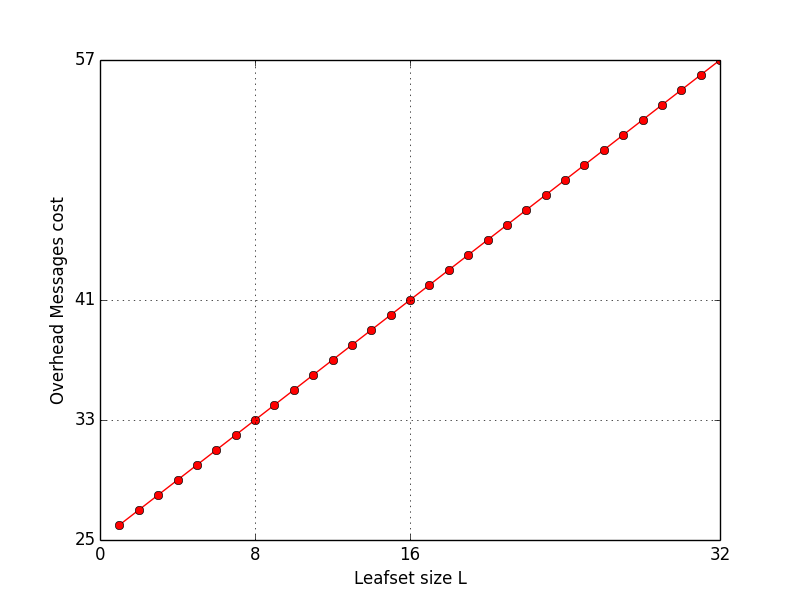
\includegraphics[width=14cm]{../plots/secure_routing_messages}\\
%\caption{Message overhead of the secure trusted routing with various sizes of Q}
%\label{fig:secure_routing_messages}
%\end{figure}




%\section{Normal service request}
\label{sec:eval_service_request}
  \begin{table}
    \centering
    \footnotesize
    \begin{tabular}{|c|c|c|}
      \cline{2-3}
      \multicolumn{1}{c|}{}&  \multicolumn{2}{c|}{\textbf{Probability to fail}} \\ \cline{2-3}
      \hline
      \textbf{Size of Trusted Set (L)} & \textbf{p = 0.3} & \textbf{p = 0.05} \\
      \hline \hline
      8 &  $0.188$ & $6.64 \times 10^{-5}$ \\
      \hline
      16 & $0.079$ & $6.57 \times 10^{-8}$  \\
      \hline
      32 & $0.016$ & $8.24 \times 19^{-14}$  \\
      \hline
    \end{tabular}
    \caption{Probability of failure when doing a normal service request}
    \label{tab:p_service_request}
  \end{table}
  
  \begin{enumerate}
    \item{\textit{Probability of failure:}}
    The user registration between a node $A$ and $S$ can fail (a) if $S$does
not respond to $A$ during the registration request or during the registration
progress, or (b) if $S$ does not send the ACKs to $A$ to terminate the user
registration. In both cases, this corresponds to the probability that more than
$L/2$ nodes of $S$ are malicious. The probability of encountering exactly $k$
malicious nodes among $L +1$ is given by the binomial distribution

    \begin{equation}
      P_{K malicious} = \begin{pmatrix} L+1 \\ k\end{pmatrix} p^k (1-p)^{L+1-k}
    \end{equation}

    where $p$ is the probability that a single node is malicious. Hence the
probability of facing at most k malicious nodes is 

    \begin{equation}
      P_{\leq k} = \sum_{i=1}^{k} \begin{pmatrix} L+1 \\ k\end{pmatrix} p^i (1-p)^{L+1-i}
    \end{equation}

    Therefore, the probability of facing more than $k$ malicious nodes among
$n$ is given by

    \begin{equation}
      P_{\ge k} = P_{\leq n} - P_{\leq k}
    \end{equation}

    and the probability that $S$ will not respond is

    \begin{align}
      P_{\ge L/2} &= P_{\leq L+1} - P_{\leq L/2} \\
      &= \sum_{i=1}^{L+1} \begin{pmatrix} L+1 \\ i\end{pmatrix} p^i (1-p)^{L+1-i}
      - \sum_{i=1}^{L/2} \begin{pmatrix} L+1 \\ i\end{pmatrix} p^i (1-p)^{L+1-i}
    \end{align}

    %% TODO: figure with the likeliness of dealing with an increains gnumber k of malicious nodes among a leafset comprising 32 nodes.

    Then the probability that $S$ will not respond to the user registration
request or to not send the final ACKs is

    \begin{align}
      P_{AS} &= (1- P_{\ge L/2}) P_{\ge L/2} +  P_{\ge L/2} \\
      P_{AS} &= 2P_{\ge L/2}) + P^2_{\ge L/2}
    \end{align}


    Table~\eqref{tab:p_account_registration} shows the probability of failure
between $A$ and $S$, for a leafset size of $L = \{8,16,32\}$.

    
    \item{\textit{Message complexity:}}
    First, $A$ must get the leafset of $S$. The associated cost is $n = 5
\times O(log_{2b}(N)) + Q + 4$ (as seen in section~\ref{sec:eval_leafset}).
    The number $n$ of message inherent to the transaction itself is given by

    \begin{align}
      n &= \underbrace{2(L+1)}_\text{Init} \underbrace{r(L+1)}_\text{Data} \underbrace{L+1}_\text{ACKs}\\
      n &= (r+3)(L+1)
    \end{align}
    where $r$ corresponds to the number of data messages sent by $A$ to $S$,
and fully depends on the transaction. The total cost is then

    $$
      n_{total} = 5 \times O(log_{2b}(N)) + Q + 4 + (r+3)(L+1)
    $$    
    The total cost only depends on the size $L$ of the leafset, which is a
constant, and $O(log(N))$. In the best case, 

    $$
      n_{total} = O(log_{2b}(N)) + (r+3)(L+1)
    $$
    Therefore, the cost of a transaction between $A$ and service $S$ remains
scalable when the size $N$ of the DHT increases.

  \end{enumerate}


\section{Account registration}
\label{sec:eval_account_registration}
  % TODO Recalculate table
  \begin{table}
    \centering
    \footnotesize
    \begin{tabular}{|c|c|c|}
      \cline{2-3}
      \multicolumn{1}{c|}{}&  \multicolumn{2}{c|}{\textbf{Probability to fail}} \\ \cline{2-3}
      \hline
      \textbf{Size of Trusted Set (L)} & \textbf{$p = \rho$ = 0.3} & \textbf{$p = \varepsilon$ = 0.05} \\
      \hline \hline
      %8 &  $0.0988087$ & $3.32222 \times 10^{-5}$ \\
      %\hline
      %16 & $0.0402769$ & $3.28714 \times 10^{-8}$  \\
      %\hline
      %32 & $0.00782066$ & $4.11893 \times 10^{-14}$  \\

      8 &  $0.098$ & $3.322 \times 10^{-5}$ \\
      \hline
      16 & $0.040$ & $3.287 \times 10^{-8}$  \\
      \hline
      32 & $0.007$ & $4.118 \times 10^{-14}$  \\
      \hline
    \end{tabular}
    \caption{Probability of failure when registering a new user account}
    \label{tab:p_account_registration}
  \end{table}
  
  \subsection{Probability of failure}
    The user registration between a node $A$ and $I$ can fail if $I$ does
not respond (or responds false information) to $A$ during the registration request or during the registration
progress. In all cases, this corresponds to the probability that more than
$L/2$ nodes of $I$ are malicious. The probability of encountering exactly $k$
malicious nodes among $L +1$ is given by the binomial distribution

    \begin{equation} \label{eq:p_k_malicious_nodes}
      P_{K malicious} = \begin{pmatrix} L+1 \\ k\end{pmatrix} p^k (1-p)^{L+1-k}
    \end{equation}

    where $p$ is the probability that a single node is malicious. Hence the
probability of facing at most k malicious nodes is 

    \begin{equation}
      P_{\leq k} = \sum_{i=1}^{k} \begin{pmatrix} L+1 \\ k\end{pmatrix} p^i (1-p)^{L+1-i}
    \end{equation}

    Therefore, the probability of facing more than $k$ malicious nodes among
$n$ is given by

    \begin{equation} \label{eq:p_malicious_ge_k}
      P_{\ge k} = P_{\leq n} - P_{\leq k}
    \end{equation}

    and the probability that $I$ will not respond is

    %% for wolfram alpha
    %% P_{\leq L+1} =  sum( ((L+1) choose i)  * p^i * (1-p)^(L+1-i), from i=1 to L+1) where L=8, p=0.3
    %% P_{\ge L/2}  =  sum( ((L+1) choose i)  * p^i * (1-p)^(L+1-i), from i=1 to L+1) - sum( ((L+1) choose i)  * p^i * (1-p)^(L+1-i), from i=1 to L/2)  where L=8, p=0.3

    \begin{align} \label{eq:p_malicious_ge_L_2}
      P_{\ge L/2} &= P_{\leq L+1} - P_{\leq L/2} \\
      &= \sum_{i=1}^{L+1} \begin{pmatrix} L+1 \\ i\end{pmatrix} p^i (1-p)^{L+1-i}
      - \sum_{i=1}^{L/2} \begin{pmatrix} L+1 \\ i\end{pmatrix} p^i (1-p)^{L+1-i}
    \end{align}

    %% TODO: figure with the likeliness of dealing with an increains gnumber k of malicious nodes among a leafset comprising 32 nodes.

    Then the probability that $I$ will not respond to the user registration
request or responds with a fake registration response is

    \begin{align}
      P_{AI} &= P_{\ge L/2} 
    \end{align}


    Table~\eqref{tab:p_account_registration} shows the probability of failure
between $A$ and $I$, for a leafset size of $L = \{8,16,32\}$. The probability
of an node failing in a system that does not implement the reputation system
is, in the best case with $L=32$, very high ($0.007$). This probability is not
acceptable for a real life system.  By using a reputation system, the probability greatly
improved in more than 5 orders of magnitude in comparison with the
non-reputation system case. With $L=16$, using a reputation system, we attain
a low probability of the order $10^{-8}$, and by using $L=32$ we get a very low
probability of $4.118 \times 10^{-14}$. If we calculate the number of
errors in a million of transactions with a probability of error of $4.118
\times 10^{-14}$, none of them should fail ($0.0000004118$ failures). This probability
makes errors almost non-existent, and should be the ideal amount for systems of with
millions of nodes that wants to prioritize their security.

    
  \subsection{Message complexity}

    First, $A$ must get the leafset of $I$. The associated cost is $5
\times O(log_{2b}(N)) + Q + 4$ (as seen in section~\ref{sec:eval_leafset}).
    The number $n$ of message inherent to the transaction itself is given by

    \begin{align}
      n &= \underbrace{2(L+1)}_\text{Init} +
           \underbrace{L+1}_\text{Registration Data} +
           \underbrace{(L+2)(L+1)}_\text{Challenge} +
           \underbrace{(L+1)L}_\text{I registration confirmations} +
           \underbrace{L+1}_\text{ACKs}\\
      n &= (2L+6)(L+1)\\
      n &= 2L^2+ 8L + 6
    \end{align}

     The total cost is then
    $$
      n_{total} = 5 \times O(log_{2b}(N)) + Q + 4 + 2L^2 + 8L + 6
    $$    

    The total cost only depends on the size $L$ of the leafset, which is a
constant, and $O(log(N))$. In the best case, 
    $$
      n_{total} = O(log_{2b}(N)) + 2L^2 + 8L + 6
    $$

    We show in table~\ref{tab:registration_messages} the number of messages sent at
    the account registration protocol with different values of $L$. In a DHT with
    $L = 16$, our system sends $671$ messages, with a failure probability of
    order $3.287 \times 10^{-8}$. If we increase the leafset size $L$ to $32$, the amount of
    messages goes up to $2335$ with a failure probability of $4.118 \times 10^{-14}$.
  
    As $L$ is a fixed value, independent of the network size $N$, the cost user
    registration operation remains scalable when the
    size $N$ of the DHT increases. While there is a high constant cost that
    depends of the number of $L$, this operation is not made frequently
    in the network and should not affect the performance of the
    service.

%\begin{figure}[!htb]
%\centering
%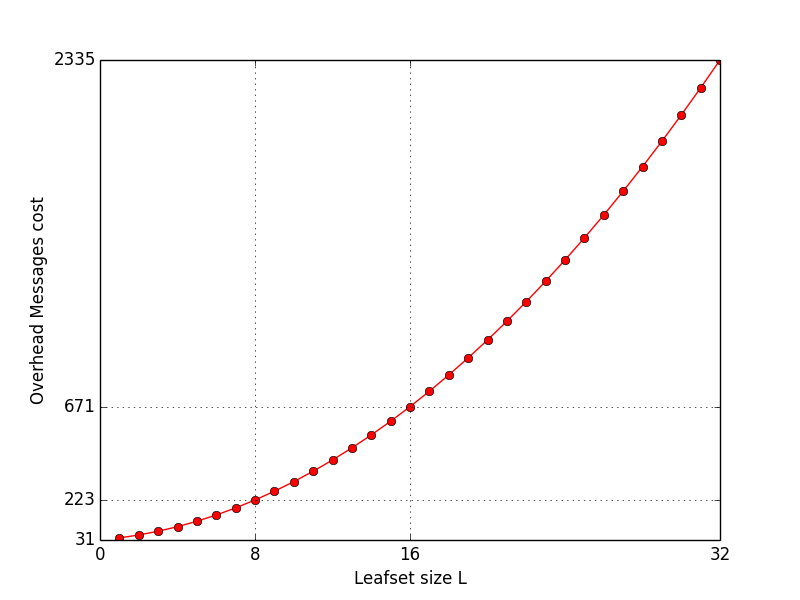
\includegraphics[width=14cm]{../plots/account_registration_messages}\\
%\caption{Message overhead of the registration protocol with various sizes of L}
%\label{fig:registration_messages}
%\end{figure}

\begin{table}
  \centering
  \footnotesize
  \begin{tabular}{|c|c|}
    \hline
     \textbf{Leafset size L} & \textbf{Message overhead}\\
    \hline
      $L = 8$ & $223$\\
    \hline
      $L = 16$ & $671$\\
    \hline
      $L = 32$ & $2335$\\
    \hline
  \end{tabular}
  \caption{Message overhead of the registration protocol with various sizes of L}
  \label{tab:registration_messages}
\end{table}


%\section{Lazy User's Information Store Maintenance}
%\label{sec:eval_lazy_maintenance}
%
%      %8 &  $0.0988087$ & $3.32222 \times 10^{-5}$ \\
%      %\hline
%      %16 & $0.0402769$ & $3.28714 \times 10^{-8}$  \\
%      %\hline
%      %32 & $0.00782066$ & $4.11893 \times 10^{-14}$  \\
%
%  \begin{table}
%    \centering
%    \footnotesize
%    \begin{tabular}{|c|c|c|c|}
%      \cline{3-4}
%      \multicolumn{2}{c|}{} &  \multicolumn{2}{c|}{\textbf{Probability to fail}} \\ \cline{2-3}
%      \cline{2-4}
%      \multicolumn{1}{c|}{} & \textbf{L} & \textbf{$p = \rho$ = 0.3} & \textbf{p = 0.05} \\
%      \hline
%      \multirow{3}{*}{\rotatebox[origin=c]{90}{\textbf{Case 1}}} & 8 & $0.106108$ & $3.9472 \times 10^{-5}$\\
%      \cline{2-4}
%      \multicolumn{1}{|c|}{} & 16 & $0.0403399$ & $3.29105 \times 10^{-8}$ \\
%      \cline{2-4}
%      \multicolumn{1}{|c|}{} & 32 & $0.00782066$ & $4.11893 \times 10^{-14}$ \\
%      \hline
%      \multirow{3}{*}{\rotatebox[origin=c]{90}{\textbf{Case 2}}} & 8 & $0.123141$ & $1.58218 \times 10^{-4}$ \\
%      \cline{2-4}
%      \multicolumn{1}{|c|}{} & 16 & $0.0404868$ & $3.36526 \times 10^{-8}$ \\
%      \cline{2-4}
%      \multicolumn{1}{|c|}{} & 32 & $0.00782067$ & $4.11893 \times 10^{-14}$ \\
%      \hline
%    \end{tabular}
%    \caption{Probability of failure when performing the user's information store maintenance}
%    \label{tab:p_lazy_maintenance}
%  \end{table}
%  
%  \subsection{Probability of failure}
%
%    We must consider two cases for certificate log maintenance: when a new node
%enters the leafset (case 1) and when a node leaves the leafset (case 2).
%
%    \paragraph{\textbf{Case 1}} A new node enters the leafset. The maintenance
%of the user information fails if it encounters $\frac{L}{2}$ consecutive
%malicious nodes when building the node interval to retrieve the logs, or if
%more than $\frac{L}{2}$ nodes are malicious (impossibility to have more than
%$\frac{L}{2} +1$ identical answers).\\
%    The probability $P_1$ of having $\frac{L}{2}$ consecutive malicious nodes
%is given by equation~\ref{eq:p_k_malicious_nodes}: $P_1 = p^{L/2}$, and the
%probability $P_2$ of not being able to retrieve at least $\frac{L}{2} +1$
%identical answers is given by equation~\ref{eq:p_malicious_ge_L_2}: $P_2 =
%P_{\ge L/2}$.\\
% Hence the total probability that this maintenance operation will
%fail is
%
%$$
%  P_{total} = P_1 + (1-P_1) P_2
%$$
%
%
%    \paragraph{\textbf{Case 2}} A node is leaving the leafset. The user
%information cannot be repaired if the node cannot repair its leafset (adding a
%node on the left or right side), or if it is impossible to find at least
%$\frac{L}{2} +1$ identical answers to retrieve the user information.
%
%A node cannot repair its leafset if $\frac{L}{2} -1$ consecutive nodes are
%malicious with a probability $P_1 = p^{L/2 - 1}$ and the user information
%retrieval fails with a probability $P_2 = P_{\ge L/2}$.\\
%Hence the total probability of failure is
%$$
%  P_{total} = P_1 + (1-P_1)P_2
%$$
%
%Table~\ref{tab:p_lazy_maintenance} computes the probability that a maintenance
%operation will fail, given increasing leafset sizes $L = {8,16,32}$.


\section{User Sign in}
\label{sec:eval_sign_in}
  \begin{table}
    \centering
    \footnotesize
    \begin{tabular}{|c|c|c|}
      \cline{2-3}
      \multicolumn{1}{c|}{}&  \multicolumn{2}{c|}{\textbf{Probability to fail}} \\ \cline{2-3}
      \hline
      \textbf{Size of Trusted Set (L)} & \textbf{$p = \rho$ = 0.3} &  \textbf{$p = \varepsilon$ = 0.05} \\
      \hline \hline
      8 &  $0.188$ & $6.64 \times 10^{-5}$ \\
      \hline
      16 & $0.079$ & $6.57 \times 10^{-8}$  \\
      \hline
      32 & $0.016$ & $8.24 \times 10^{-14}$  \\
      \hline
    \end{tabular}
    \caption{Probability of failure in user sign-in}
    \label{tab:p_sign_in}
  \end{table}
  
  \subsection{Probability of failure}
    A sign-in request between a node $A$ and the service $S$, can fail (a) if the identification service $I$ does
not respond (or responds fake information) to $S$ during the user information recovery
request, or (b) if $S$ does not respond (or responds fake information) to $A$
during the challenge or the session keys generation. While a response with fake information can be more dangerous for the
user, the probability remains the same, corresponding to the
probability that more than $L/2$ nodes of $I$ (or $S$) are malicious.
    As seen before, the probability of facing more than $k$ malicious nodes among
$n$ is given by the equation~\ref{eq:p_k_malicious_nodes}.

    Then the probability that $I$ will not respond to the service user
information recovery request, or that $S$ not respond to the node $A$ is

    \begin{align}
      P_{AI} &= (1- P_{\ge L/2}) P_{\ge L/2} +  P_{\ge L/2} \\
      P_{AI} &= 2P_{\ge L/2} - P^2_{\ge L/2}
    \end{align}


    Table~\eqref{tab:p_sign_in} shows the probability of failure
between $A$, the service $S$ and $I$, for a leafset size of $L = \{8,16,32\}$.
    The probability of the protocol failing without using a reputation system
is very high. If we take the best case with $L=32$, the probability is around
16 nodes failing out of 1000. On the other hand, using a reputation system we
get pretty good results, with an order of $10^{-8}$ using $L=16$ and an order
of $10^{-14}$ with $L=32$, a very low probability. Both of them can be used
in real life scenario, with $L=32$ being the most secure of them all.

  \subsection{Message complexity}

    First, $A$ must get the leafset of $S$. The associated cost is $5
\times O(log_{2b}(N)) + Q + 4$ (as seen in section~\ref{sec:eval_leafset}).
Then, every node in $S$ must get the leafset of $I$, with each leafset request
having the same associated cost as before $n = (L+1)(5 \times O(log_{2b}(N)) + Q + 4)$~\ref{sec:eval_leafset}.
    The number $n$ of message inherent to the transaction itself is given by

    \begin{align}
      % TODO: + ommited for space, fix this with other way to express this
      n &= \underbrace{2(L+1)}_\text{Init A with S} +
           \underbrace{2(L+1)^2}_\text{Init S with I} +
           \underbrace{(L+1)^2}_\text{Data from I to S} +
           \underbrace{(L+1)L}_\text{Init Challenge} +
           \underbrace{2(L+1)}_\text{S challenges A} +
           \underbrace{L+1}_\text{ACKs}\\
      n &= 5(L+1) + 3(L+1)(L+1)+ (L+1)L\\
      n &= 4L^2 +12L + 8 
    \end{align}
     The total cost is then

    $$
      n_{total} = (L +2)(5 \times O(log_{2b}(N)) + Q + 4) + 4L^2 +12L + 8 
    $$    
    The total cost only depends on the size $L$ of the leafset, which is a
constant, and $O(log(N))$. In the best case, 

    $$
      n_{total} = (L +2)O(log_{2b}(N)) + 4L^2 +12L + 8 
    $$

    Therefore, the cost of a user sign in operation remains
scalable when the size $N$ of the DHT increases.

    We show in table~\ref{tab:sign_in_messages} the number of messages sent at
the sign in protocol with different values of $L$. In a DHT with
$L = 16$, our system sends $1890$ messages, with a failure probability of
 $6.57 \times 10^{-8}$. If we increase the leafset size $L$ to $32$, the amount of
messages goes up to $5746$ with a failure probability of $8.24 \times 10^{-14}$.


%\begin{figure}[!htb]
%\centering
%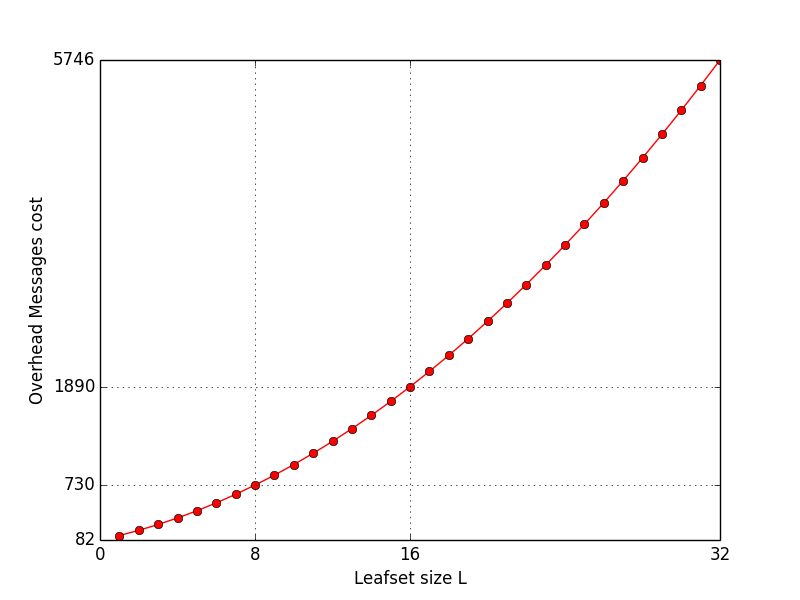
\includegraphics[width=14cm]{../plots/sign_in_messages}\\
%\caption{Message overhead of the sign in protocol with various sizes of L}
%\label{fig:sign_in_messages}
%\end{figure}

\begin{table}
  \centering
  \footnotesize
  \begin{tabular}{|c|c|}
    \hline
     \textbf{Leafset size L} & \textbf{Message overhead}\\
    \hline
      $L = 8$ & $730$\\
    \hline
      $L = 16$ & $1890$\\
    \hline
      $L = 32$ & $5746$\\
    \hline
  \end{tabular}
  \caption{Message overhead of the sign in protocol with various sizes of L}
  \label{tab:sign_in_messages}
\end{table}


\section{Logout}
  \label{sec:eval_logout}
  \begin{table}
    \centering
    \footnotesize
    \begin{tabular}{|c|c|c|}
      \cline{2-3}
      \multicolumn{1}{c|}{}&  \multicolumn{2}{c|}{\textbf{Probability to fail}} \\ \cline{2-3}
      \hline
      \textbf{Size of Trusted Set (L)} & \textbf{$p = \rho$ = 0.3} &  \textbf{$p = \varepsilon$ = 0.05} \\
      \hline \hline
      8 &  $0.098$ & $3.322 \times 10^{-5}$ \\
      \hline
      16 & $0.040$ & $3.287 \times 10^{-8}$  \\
      \hline
      32 & $0.007$ & $4.118 \times 10^{-14}$  \\
      \hline
    \end{tabular}
    \caption{Probability of failure in user logout}
    \label{tab:p_logout}
  \end{table}
  
  \subsection{Probability of failure}
    The user logout between a node $A$ and $S$ can fail if $S$ does
not respond (or responds false information) to $A$ during the logout request.
  In all cases, this corresponds to the probability that more than
$L/2$ nodes of $I$ are malicious.
    As seen before, the probability of facing more than $k$ malicious nodes among
$n$ is given by the equation~\ref{eq:p_k_malicious_nodes}.\\

    Then the probability that $S$ will not respond to the user logout 
request or responds with a fake logout response is

    \begin{align}
      P_{AI} &= P_{\ge L/2} 
    \end{align}


    Table~\eqref{tab:p_logout} shows the probability of failure
between $A$ and $S$, for a leafset size of $L = \{8,16,32\}$.
  The probability distribution results the same obtained as the registration
protocol~\ref{sec:eval_account_registration} seen before, and the same analysis
can be applied to it. The probability
of an node failing in a system that does not implement the reputation system
is, in the best case with $L=32$, very high ($0.007$). This probability is not
acceptable for a real life system.  By using a reputation system, the probability greatly
improved in more than 5 orders of magnitude in comparison with the
non-reputation system case. With $L=16$, using a reputation system, we attain
a low probability of the order $10^{-8}$, and by using $L=32$ we get a very low
probability of $4.118 \times 10^{-14}$. If we calculate the number of
errors in a million of transactions with a probability of error of $4.118
\times 10^{-14}$, none of them should fail ($0.0000004118$ failures). This probability
makes errors almost non-existent, and should be the ideal amount for systems of with
millions of nodes that wants to prioritize their security.

    
  \subsection{Message complexity}
    First, $A$ must get the leafset of $S$. The associated cost is $5
\times O(log_{2b}(N)) + Q + 4$ (as seen in section~\ref{sec:eval_leafset}).
    The number $n$ of message inherent to the transaction itself is given by

    \begin{align}
      n &= \underbrace{2(L+1)}_\text{Init} +  \underbrace{L+1}_\text{Logout Request} + \underbrace{L+1}_\text{ACKs}\\
      n &= 4(L+1)
    \end{align}
     The total cost is then

    $$
      n_{total} = 5 \times O(log_{2b}(N)) + Q + 4 + 4(L+1)
    $$    
    The total cost only depends on the size $L$ of the leafset, which is a
constant, and $O(log(N))$. In the best case, 

    $$
      n_{total} = O(log_{2b}(N)) + 4(L+1)
    $$
    Therefore, the cost of a user logout operation remains scalable when the size $N$ of the DHT increases.

    We show in table~\ref{tab:logout_messages} the number of messages sent at
the logout protocol with different values of $L$. In a DHT with
$L = 16$, our system sends $105$ messages, with a failure probability of
 $3.287 \times 10^{-8}$. If we increase the leafset size $L$ to $32$, the amount of
messages goes up to $169$ with a failure probability of $4.118 \times 10^{-14}$.


%\begin{figure}[!htb]
%\centering
%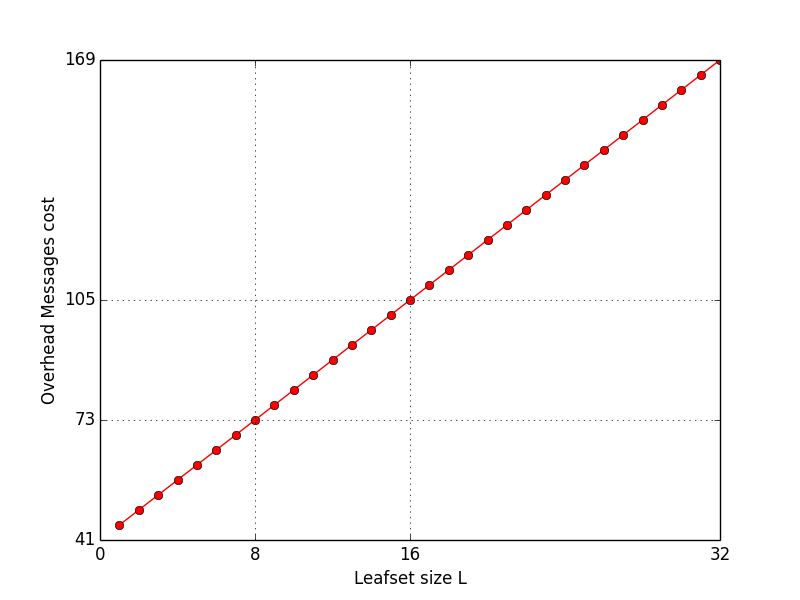
\includegraphics[width=14cm]{../plots/logout_messages}\\
%\caption{Message overhead of the logout protocol with various sizes of L}
%\label{fig:logout_messages}
%\end{figure}

\begin{table}
  \centering
  \footnotesize
  \begin{tabular}{|c|c|}
    \hline
     \textbf{Leafset size L} & \textbf{Message overhead}\\
    \hline
      $L = 8$ & $73$\\
    \hline
      $L = 16$ & $105$\\
    \hline
      $L = 32$ & $169$\\
    \hline
  \end{tabular}
  \caption{Message overhead of the logout protocol with various sizes of L}
  \label{tab:logout_messages}
\end{table}

\section{Password Change}
  \label{sec:eval_password_change}
  \begin{table}
    \centering
    \footnotesize
    \begin{tabular}{|c|c|c|}
      \cline{2-3}
      \multicolumn{1}{c|}{}&  \multicolumn{2}{c|}{\textbf{Probability to fail}} \\ \cline{2-3}
      \hline
      \textbf{Size of Trusted Set (L)} & \textbf{$p = \rho$ = 0.3} &  \textbf{$p = \varepsilon$ = 0.05}  \\
      \hline \hline
      8 &  $0.098$ & $3.322 \times 10^{-5}$ \\
      \hline
      16 & $0.040$ & $3.287 \times 10^{-8}$  \\
      \hline
      32 & $0.007$ & $4.118 \times 10^{-14}$  \\
      \hline
    \end{tabular}
    \caption{Probability of failure when changing the user password}
    \label{tab:p_password_change}
  \end{table}
  
  \subsection{Probability of failure}
    A password change request between a node $A$, the identification service
$I$ can fail (a) if $L/2 + 1$ nodes in $I$ does not responds (or responds fake
information) correctly the password change confirmation message to the nodes 
$I_i \in I$ during the password change request, or (b) if $S$ does not respond (or responds fake information) to $A$
during the password change request. While a response with fake information can be more dangerous for the
user, the event of that happening is the same as when there is no response:
when more than $L/2$ nodes of $I$ are malicious.

    As seen before, the probability of facing more than $k$ malicious nodes among
$n$ is given by the equation~\ref{eq:p_k_malicious_nodes}.\\

    Then the probability that $I$ will not respond to the service user
information recovery request is

    \begin{align}
      P_{AI} &= P_{\ge L/2}
    \end{align}


    Table~\eqref{tab:p_password_change} shows the probability of failure
between $A$, the service $S$ and $I$, for a leafset size of $L = \{8,16,32\}$.
Maintains the same distribution as the user registration
protocol~\ref{sec:eval_account_registration} and the
logout protocol seen before~\ref{sec:eval_logout}.

  \subsection{Message complexity}

    First, $A$ must get the leafset of $I$. The associated cost is $5
\times O(log_{2b}(N)) + Q + 4$ (as seen in section~\ref{sec:eval_leafset}).
%%% not needed, this has to be done in the leafset maintenance
%Then, every node in $I$ must get the leafset of $I$, with each leafset request
%having the same associated cost as before $n = (L+1)(5 \times O(log_{2b}(N)) + Q + 4)$~\ref{sec:eval_leafset}.
    The number $n$ of message inherent to the transaction itself is given by

    \begin{align}
      n &= \underbrace{2(L+1)}_\text{Init A with I} +
           \underbrace{(L+1)L}_\text{Data from I to I} +
           \underbrace{L+1}_\text{ACKs}\\
      n &= 3(L+1) + L(L+1)\\
      n &= L^2 + 4L + 3
    \end{align}
     The total cost is then

    $$
      n_{total} = 5 \times O(log_{2b}(N)) + Q + 4 +  L^2 + 4L + 3
    $$    
    The total cost only depends on the size $L$ of the leafset, which is a
constant, and $O(log(N))$. In the best case, 

    $$
      n_{total} = O(log_{2b}(N)) + L^2 + 4L + 3
    $$
    Therefore, the cost of a password change operation remains
scalable when the size $N$ of the DHT increases.

    We show in table~\ref{tab:password_change_messages} the number of messages sent at
the password change protocol with different values of $L$. In a DHT with
$L = 16$, our system sends $360$ messages, with a failure probability of
 $3.287 \times 10^{-8}$. If we increase the leafset size $L$ to $32$, the amount of
messages goes up to $1192$ with a failure probability of $4.118 \times 10^{-14}$.

%\begin{figure}[!htb]
%\centering
%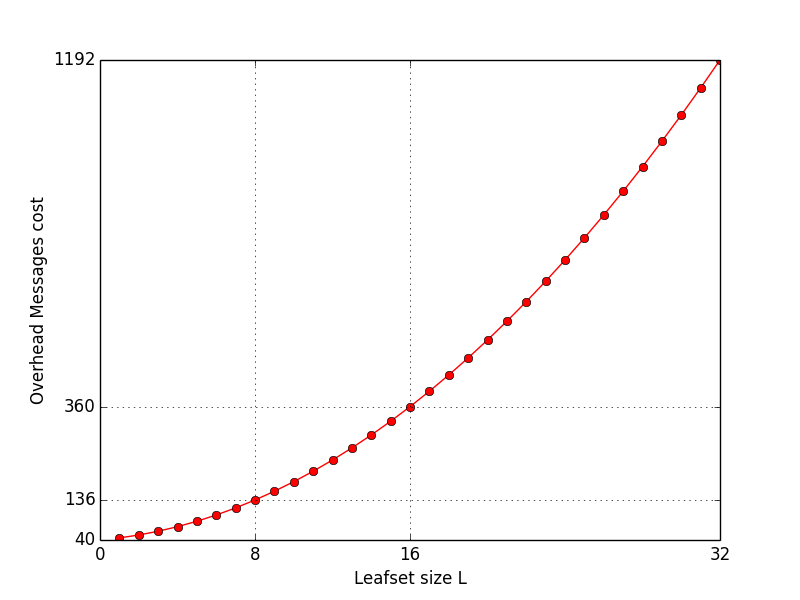
\includegraphics[width=14cm]{../plots/password_change_messages}\\
%\caption{Message overhead of the password change protocol with various sizes of L}
%\label{fig:password_change_messages}
%\end{figure}

\begin{table}
  \centering
  \footnotesize
  \begin{tabular}{|c|c|}
    \hline
     \textbf{Leafset size L} & \textbf{Message overhead}\\
    \hline
      $L = 8$ & $136$\\
    \hline
      $L = 16$ & $360$\\
    \hline
      $L = 32$ & $1192$\\
    \hline
  \end{tabular}
  \caption{Message overhead of the password change protocol with various sizes of L}
  \label{tab:password_change_messages}
\end{table}

%We suppose in the following that the underlying
%reputation system makes an error $p = \varepsilon$ when classifying a
%node $X$ with a reputation $R(x) \geq p = \rho$, where $p = \rho \in [ 0 \cdots 1 ]$,
%and $ p = \varepsilon = f ( p = \rho )$. In other words, classifying a node $X$ as
%honest because its reputation is greater than $p = \rho$ has a
%probability of error $p = \varepsilon$.
%Let $n$ be the size of the Trusted Ring. The probability
%to have $k$ misclassified nodes in the Trusted Ring, that
%is $k$ malicious nodes is:
%
%$$
%P_{k_{malicious}} = \left(\!
%                          \begin{array}{c}
%                            n\\
%                            k
%                          \end{array}
%                    \!\right)              
%                    p = \varepsilon^{n-k} ( 1 - p = \varepsilon )^k
%$$
%
%Then, the probability to have at most $k$ malicious
%nodes in a Trusted Ring of size $n$ is:
%
%$$
%P_{\leq k} = \sum^{k}_{i=1} \left(\!
%                                \begin{array}{c}
%                                    n\\
%                                    k
%                                  \end{array}
%                            \!\right)              
%                    p = \varepsilon^{n-i} ( 1 - p = \varepsilon )^i
%$$
%
%Therefore, the probability to have $k$ or more malicious
%nodes in a Trusted Ring of size $n$ is:
%
%$$
%P_{\leq k} = \sum^{n}_{i=k} \left(\!
%                                \begin{array}{c}
%                                    n\\
%                                    i
%                                  \end{array}
%                            \!\right)              
%                    p = \varepsilon^{n-i} ( 1 - p = \varepsilon )^i
%$$
%
%The user identification fails when:
%\begin{enumerate}
%  \item The user cannot retrieve his own PKI from the \textit{trustset}.
%  \item or when the public key of the user fails to be retrieved.
%\end{enumerate}
%
%These failures can happen when the \textit{trustsets} storing the PKI or the public
%key have more malicious nodes than normal nodes.
%
%The probability that a \textit{trustset} has half or more malicious nodes, assuming a maximum
%classification error for the underlying reputation system
%of $5\%$, is .% FILL HERE
%%Hence the probability for having a fully erroneous trustset is theoretically possible, but
%%practically infeasible.
%
%Considering a maximum error rate of $5\%$ is a typical
%value for a reputation system. In some cases it may be
%over-estimated (for more details, please refer the results
%obtained for the WTR reputation system\cite{wrt_reputation_system}). This
%error hardly depends on the total number of malicious
%nodes in the network, and decreases when the ratio
%of malicious node decreases. The less malicious nodes
%there are in the system, the easier it is to discriminate
%against them.

\section{User private key recovery}
\label{sec:eval_private_key_recovery}
% TODO Recalculate table
  \begin{table}
    \centering
    \footnotesize
    \begin{tabular}{|c|c|c|}
      \cline{2-3}
      \multicolumn{1}{c|}{}&  \multicolumn{2}{c|}{\textbf{Probability to fail}} \\ \cline{2-3}
      \hline
      \textbf{Size of Trusted Set (L)} & \textbf{$p = \rho$ = 0.3} &  \textbf{$p = \varepsilon$= 0.05} \\
      \hline \hline
      8 &  $0.098$ & $3.322 \times 10^{-5}$ \\
      \hline
      16 & $0.040$ & $3.287 \times 10^{-8}$  \\
      \hline
      32 & $0.007$ & $4.118 \times 10^{-14}$  \\
      \hline
    \end{tabular}
    \caption{Probability of failure when recovering user private key}
    \label{tab:p_private_key_recovery}
  \end{table}

  \subsection{Probability of failure}

    The user private key recovery between a node $A$ and the leafset of the
node $T$ can fail (a) if the leafset of $T$ does
not respond (or responds fake information) to $A$ during the key recovery
request, where $T$ is the node in charge of the storage of the key $K=
SHA(U^{username}) + SHA(U^{password})$. While a response with fake information (like a salt forged by malicious nodes) can be more dangerous for the
user, the probability remains the same, corresponding to the
probability that more than $L/2$ nodes of $T$ are malicious.\\
    The probability that the leafset of $T$ will not respond to the user private key recovery
request (or that the leafset of $T$ responds fake user information) is the probability of
facing more than $\frac{L}{2} +1$ malicious nodes in the leafset of $T$. This probability is given by the
equation~\ref{eq:p_malicious_ge_L_2} and hence the probability that the user
private key recovery fails is:

\begin{equation} \label{eq:L_2_malicious_A_I}
 P_{AT} = P_{\ge L/2}
\end{equation}

    Table~\eqref{tab:p_private_key_recovery} shows the probability of failure
between $A$ and the leafset of $T$, for a leafset size of $L = \{8,16,32\}$.
Maintains the same distribution as the user registration
protocol~\ref{sec:eval_account_registration}, the
logout protocol~\ref{sec:eval_logout} and the password change
protocol~\ref{sec:eval_password_change} seen before.

    
  \subsection{Message complexity}


\begin{table}
  \centering
  \footnotesize
  \begin{tabular}{|c|c|}
    \hline
     \textbf{Leafset size L} & \textbf{Message overhead}\\
    \hline
      $L = 8$ & $73$\\
    \hline
      $L = 16$ & $105$\\
    \hline
      $L = 32$ & $169$\\
    \hline
  \end{tabular}
  \caption{Message overhead of the private key recovery protocol A with various sizes of L}
  \label{tab:private_key_recovery_a_messages}
\end{table}

    First, $A$ must get the leafset of $T$. The associated cost is $5
\times O(log_{2b}(N)) + Q + 4$ (as seen in section~\ref{sec:eval_leafset}).
    The number $n$ of message inherent to the transaction itself is given by

    \begin{align}
      n &= \underbrace{2(L+1)}_\text{Init} + \underbrace{L+1}_\text{Data} +  \underbrace{L+1}_\text{ACKs}\\
      n &= 4(L+1)
    \end{align}
     The total cost is then

    $$
      n_{total} = 5 \times O(log_{2b}(N)) + Q + 4 + 4(L+1)
    $$    
    The total cost only depends on the size $L$ of the leafset, which is a
constant, and $O(log(N))$. In the best case, 

    $$
      n_{total} = O(log_{2b}(N)) + 4(L+1)
    $$
    Therefore, the cost of recovering a user private key remains
scalable when the size $N$ of the DHT increases.

    We show in table~\ref{tab:private_key_recovery_a_messages} the number of messages sent at
the private key recovery protocol with different values of $L$. In a DHT with
$L = 16$, our system sends $105$ messages, with a failure probability of
 $3.287 \times 10^{-8}$. If we increase the leafset size $L$ to $32$, the amount of
messages goes up to $169$ with a failure probability of $4.118 \times 10^{-14}$.

%\begin{figure}[!htb]
%\centering
%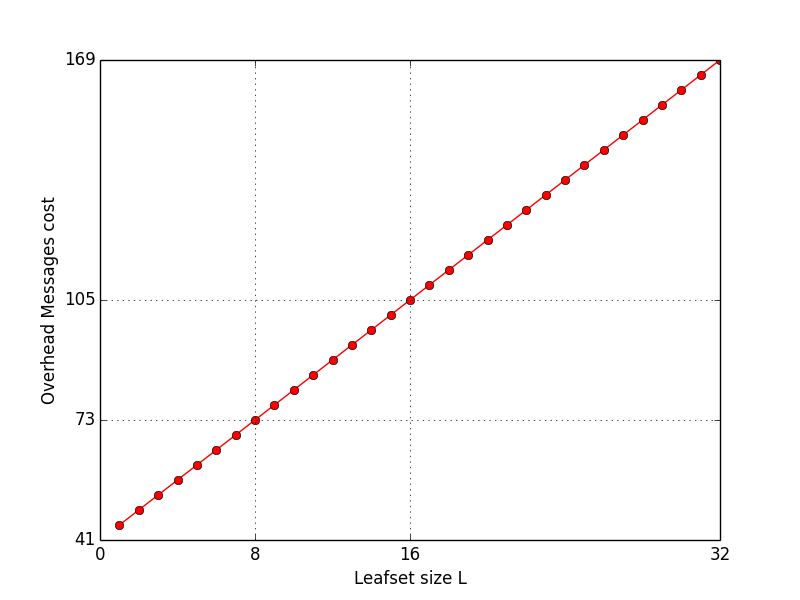
\includegraphics[width=14cm]{../plots/private_key_recovery_a_messages}\\
%\caption{Message overhead of the private key recovery protocol A with various sizes of L}
%\label{fig:private_key_recovery_a_messages}
%\end{figure}
